\documentclass{../../oss-classkick-exam}

\begin{document}
\genheader

\gentitle{8}{ROTATIONAL MOTION, PART 2}

\genmultidirections

\gengravity

\raggedcolumns
\begin{multicols*}{2}
  \begin{questions}
    \question A particle of mass $m$ moves with a constant speed $\varv$ at a
    distance $x_0$ parallel to the $y$-axis as shown. When the particle is in
    the position shown below, the magnitude of its angular momentum relative to
    the origin is
    \begin{center}
      \begin{tikzpicture}
        \fill(2,1.5) circle(.08);
        \begin{scope}[thick]
          \draw[->](-.2,0)--(3,0) node[right]{$x$} node[pos=0,below]{$O$};
          \draw[->](0,-.2)--(0,2.5) node[above]{$y$};
          \draw[dashed](0,1.5)--(2,1.5) node[pos=0,left]{$y_0$}
          --(2,0)node[below]{$x_0$};
        \end{scope}
        \draw[very thick,->](2,1.5)--(2,.5) node[midway,right]{$\varv$};
      \end{tikzpicture}
    \end{center}
    \begin{choices}
      \choice $m\varv x_0$
      \choice $m\varv y_0$
      \choice $m\varv\sqrt{x_0^2+y_0^2}$
      \choice $\dfrac{m\varv}{\sqrt{x_0^2+y_0^2}}$
      \choice zero
    \end{choices}
    
    \question A hoop of radius $R$ and mass $m$ has a rotational inertia of
    $mR^2$. The hoop rolls without slipping along a horizontal floor with a
    constant speed $\varv$ and then rolls up a long incline. The hoop can roll
    up the incline to a maximum vertical height of
    \begin{center}
      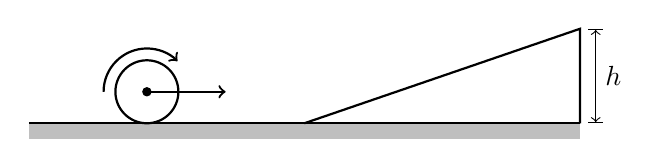
\begin{tikzpicture}
        \fill[lightgray](0,-.2) rectangle(7,0);
        \begin{scope}[thick]
          \draw(0,0)--(7,0);
          \draw(3.5,0)--(7,1.2)--(7,0);
          \draw(1.5,.4) circle(.4);
          \fill(1.5,.4) circle(.06);
          \draw[->](1.5,.4)--(2.5,.4) node[right]{$\varv$};
          \draw[->](.95,.4) arc(180:45:.55);
        \end{scope}
        \draw[|<->|](7.2,0)--(7.2,1.2) node[midway,right]{$h$};
      \end{tikzpicture}
    \end{center}
    \begin{choices}
      \choice$\dfrac{\varv^2}g$
      \choice$\dfrac{2\varv^2}{g}$
      \choice$\dfrac{\varv^2}{2g}$
      \choice$\dfrac{4\varv^2}{g}$
      \choice$\dfrac{\varv^2}{4g}$
    \end{choices}
    
    \question A disk is mounted on a fixed axle. The rotational inertia of the
    disk is $I$. The angular velocity of the disk is decreased from $\omega_i$
    to $\omega_f$ during a time $\Delta t$ due to friction in the axle. The
    magnitude of the average net torque acting on the wheel is
    \begin{choices}
      \choice $\dfrac{\omega_f-\omega_i}{\Delta t}$
      \choice $\dfrac{(\omega_f-\omega_i)^2}{\Delta t}$
      \choice $\dfrac{I(\omega_f-\omega_i)}{\Delta t}$
      \choice $\dfrac{I(\omega_f-\omega_i)^2}{\Delta t}$
      \choice $\dfrac{I(\omega_f-\omega_i)}{\Delta t^2}$
    \end{choices}
    \vspace{.7in}
    
  \question The average power developed by the friction in the axle of the disk
    from the previous question to bring it to a complete stop is
    \begin{choices}
      \choice $\dfrac{\omega_i}{\Delta t}$
      \choice $\dfrac{\omega_i^2}{\Delta t}$
      \choice $\dfrac{I\omega_i}{2\Delta t}$
      \choice $\dfrac{I\omega_i^2}{\Delta t}$
      \choice $\dfrac{I\omega_i}{\Delta t^2}$
    \end{choices}    
    \columnbreak
    
    \question Astronauts are conducting an experiment in a negligible gravity
    environment. Two spheres of mass $m$ are attached to either end of a light
    rod. As the rod and spheres float motionless in space, an astronaut
    launches a piece of sticky clay, also of mass $m$, toward one of the spheres
    so that the clay strikes and sticks to the sphere perpendicular to the rod.
    Which of the following statements is true of the motion of the rod, clay,
    and spheres after the collision?
    \begin{center}
      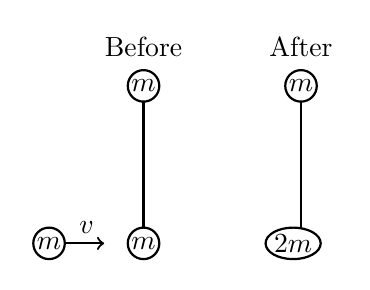
\begin{tikzpicture}
        \begin{scope}[thick]
          \draw circle(.2) node{$m$};
          \draw(0,2) circle(.2) node{$m$};
          \draw(0,.2)--(0,1.8);
          \draw(-1.2,0) circle(.2) node{$m$};
          \draw[->](-1,0)--(-.5,0) node[above left]{$v$};

          \draw(1.9,0) ellipse(.35 and .2) node{$2m$};
          \draw(2,2) circle(.2) node{$m$};
          \draw(2,.2)--(2,1.8);
        \end{scope}
        \node at (0,2.5) {Before};
        \node at (2,2.5) {After};
      \end{tikzpicture}
    \end{center}
    \begin{choices}
      \choice Linear momentum is not conserved, but angular momentum is
      conserved.
      \choice Angular momentum is not conserved, but linear momentum is
      conserved.
      \choice Kinetic energy is conserved, but angular momentum is not
      conserved.
      \choice Kinetic energy is conserved, but linear momentum is not conserved.
      \choice Both linear momentum and angular momentum are conserved, but
      kinetic energy is not conserved.
    \end{choices}
    \vspace{.7in}
    
    \question A rod of mass $M$, length $L$, and rotational inertia $I$ hangs
    at rest from a frictionless axle as shown. A ball of mass $m$ with a speed
    $\varv$ strikes therod perpendicularly at the end of the rod. As a result
    of the collision, the ball stops. The angular speed of the rod immediately
    after the collision is
    \begin{center}
      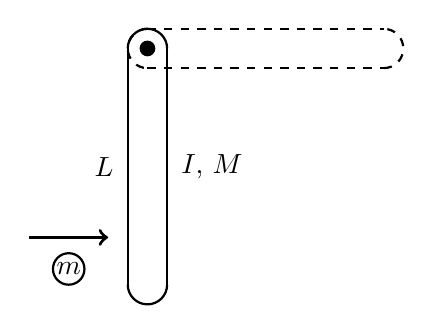
\begin{tikzpicture}
        \fill circle(.1);
        \begin{scope}[thick]
          \draw(.25,0) arc(0:180:.25);
          \draw(-.25,0)--(-.25,-3);
          \draw( .25,0)--( .25,-3);
          \draw(-.25,-3) arc(180:360:.25);
          \begin{scope}[dashed,rotate=90]
            \draw(.25,0) arc(0:180:.25);
            \draw(-.25,0)--(-.25,-3);
            \draw( .25,0)--( .25,-3);
            \draw(-.25,-3) arc(180:360:.25);
          \end{scope}
          \draw(-1,-2.8) circle(.2) node{$m$};
          \draw[very thick,->](-1.5,-2.4)--(-.5,-2.4)
          node[midway,above]{$\varv$};
          \node[left] at (-.3,-1.5) {$L$};
          \node[right] at (.3,-1.5) {$I$, $M$};
        \end{scope}
      \end{tikzpicture}
    \end{center}
    \begin{choices}
      \choice $\varv L$
      \choice $\dfrac{\varv}L$
      \choice $\dfrac{m\varv}I$
      \choice $\dfrac{m\varv L}I$
      \choice $\dfrac{m\varv}{IL}$
    \end{choices}
    \columnbreak

    \uplevel{
      \textbf{Questions \ref{hollow1}--\ref{hollow2}}

      A hollow sphere of mass $m$ and radius $R$ begins from rest at a height
      $h$ and rolls down a rough inclined plane. The rotational inertia of the
      hollow sphere is $\dfrac23mR^2$.
      \begin{center}
        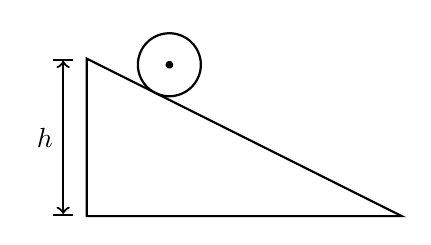
\begin{tikzpicture}
          \begin{scope}[thick]
            \draw(0,0)--(-4,0)--(-4,2)--cycle;
            \draw[|<->|](-4.3,2)--(-4.3,0) node[midway,left]{$h$};
          \end{scope}
          \begin{scope}[thick,rotate=-atan(2/4)]
            \draw(-3.5,.4) circle(.4);
            \fill(-3.5,.4) circle(.05);
          \end{scope}
        \end{tikzpicture}
      \end{center}
    }

    \question Which of the following diagrams best represents the forces acting
    on  the sphere as it rolls down the plane?
    \begin{choices}
    \choice 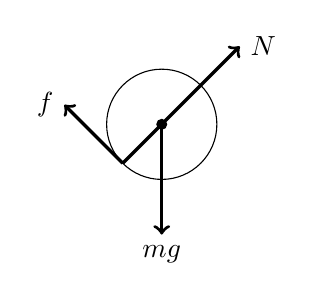
\begin{tikzpicture}[scale=.7]
      \draw circle(1);
      \fill circle(.1);
      \begin{scope}[very thick,->]
        \draw (0,0)--(0,-2) node[below]{$mg$};
        \draw[rotate=45](-1,0)--(2,0) node[right]{$N$};
        \draw[rotate=45](-1,0)--(-1,1.5) node[left]{$f$};
      \end{scope}
    \end{tikzpicture}

    \choice 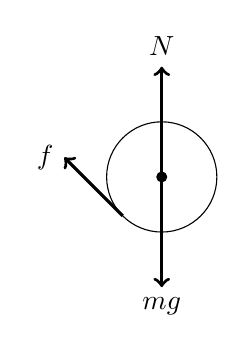
\begin{tikzpicture}[scale=.7]
      \draw circle(1);
      \fill circle(.1);
      \begin{scope}[very thick,->]
        \draw (0,0)--(0,-2) node[below]{$mg$};
        \draw (0,0)--(0,2) node[above]{$N$};
        \draw[rotate=45](-1,0)--(-1,1.5) node[left]{$f$};
      \end{scope}
    \end{tikzpicture}

    \choice 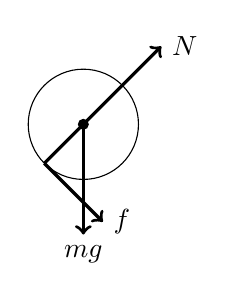
\begin{tikzpicture}[scale=.7]
      \draw circle(1);
      \fill circle(.1);
      \begin{scope}[very thick,->]
        \draw (0,0)--(0,-2) node[below]{$mg$};
        \draw[rotate=45](-1,0)--(2,0) node[right]{$N$};
        \draw[rotate=45](-1,0)--(-1,-1.5) node[right]{$f$};
      \end{scope}
    \end{tikzpicture}

    \choice 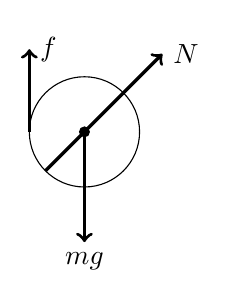
\begin{tikzpicture}[scale=.7]
      \draw circle(1);
      \fill circle(.1);
      \begin{scope}[very thick,->]
        \draw (0,0)--(0,-2) node[below]{$mg$};
        \draw[rotate=45](-1,0)--(2,0) node[right]{$N$};
        \draw(-1,0)--(-1,1.5) node[right]{$f$};
      \end{scope}
    \end{tikzpicture}
      
    \choice 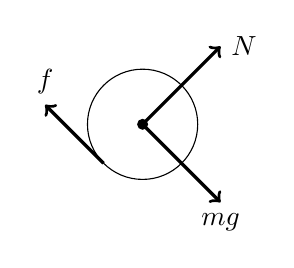
\begin{tikzpicture}[scale=.7]
      \draw circle(1);
      \fill circle(.1);
      \begin{scope}[very thick,->]
        \draw[rotate=45](0,0)--(0,-2) node[below]{$mg$};
        \draw[rotate=45](0,0)--(2,0) node[right]{$N$};
        \draw[rotate=45](-1,0)--(-1,1.5) node[above]{$f$};
      \end{scope}
    \end{tikzpicture}
    \end{choices}
    \label{hollow1}
    
    \question The speed of the sphere when it reaches the bottom of the plane is
    \begin{choices}
      \choice $\dfrac{8gh}5$
      \choice $\dfrac{6gh}5$
      \choice $\dfrac{5gh}6$
      \choice $\dfrac{7gh}{10}$
      \choice $\dfrac{gh}2$
    \end{choices}
    \label{hollow2}
    \columnbreak
    
    \question One end of a stick of length $L$, rotational inertia $I$, and
    mass $m$ is pivoted on an axle with negligible friction at point $P$. The
    other end is tied to a string and held in a horizontal position. When the
    string is cut, the stick rotates counterclockwise. The angular speed
    $\omega$ of the stick when it reaches the bottom of its swing is
    \cpic{.32}{end-of-stick}
    \begin{choices}
      \choice $\dfrac{mgL}I$
      \choice $\sqrt{\dfrac{mgL}I}$
      \choice $\sqrt{\dfrac{2mgL}I}$
      \choice $\sqrt{\dfrac{mgL}{2I}}$
      \choice $\sqrt{\dfrac{4mgL}I}$
    \end{choices}
  \end{questions}
\end{multicols*}
\newpage

\genfreetitle{8}{ROTATIONAL MOTION, PART 2}{4}

\genfreedirections

% TAKEN FROM THE 2015 AP PHYSICS C FREE-RESPONSE QUESTION MECH 3
\begin{questions}
  \question A uniform sphere of mass $M$ and radius $R$ is free to rotate,
  without friction, about a horizontal axis through its center. A string is
  wrapped around the sphere and is attached to a body of mass $m$ as shown in
  the figure below. Find
  \begin{center}
    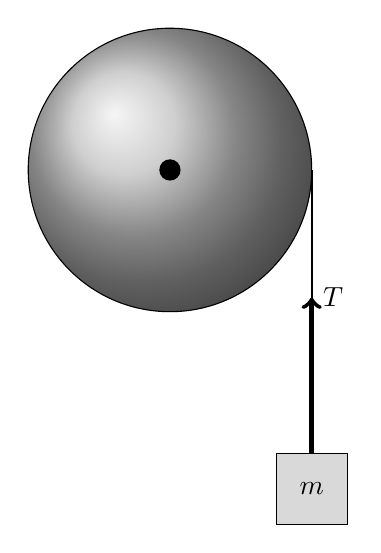
\begin{tikzpicture}[scale=.9]
      \shade[ball color=lightgray] circle (2);% node[below right]{$m$};
      \draw circle(2);
      \fill circle(.15);
      \draw[thick](2,0)--(2,-4);
      \draw[fill=gray!30](1.5,-4) rectangle(2.5,-5) node[midway]{$m$};
      \draw[ultra thick,->](2,-4)--(2,-1.8) node[right]{$T$};
    \end{tikzpicture}
  \end{center}
  \begin{parts}
    \part the acceleration of the body, and
    \part the tension in the string.
  \end{parts}
  \newpage

  \question A uniform cylinder of mass $M$ and radius $R$ has a string wrapped
  around it. The string is held fixed, and the cylinder falls vertically as
  shown in the figure below. Find
  \begin{center}
    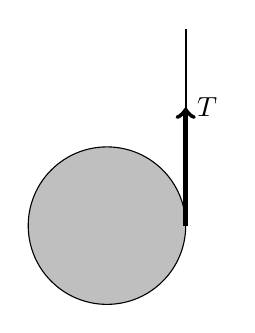
\begin{tikzpicture}[scale=.5]
      \draw[fill=lightgray] circle(2);
      \draw[thick](2,0)--(2,5);
      \draw[ultra thick,->](2,0)--(2,3) node[right]{$T$};
    \end{tikzpicture}
  \end{center}
  \begin{parts}
    \part the acceleration of the body, and
    \part the tension in the string.
  \end{parts}
  \newpage


  % TAKEN FROM THE 2004 AP PHYSICS C MECHANICS EXAM FREE-RESPONSE QUESTION 2
  \uplevel{
    \begin{center}
      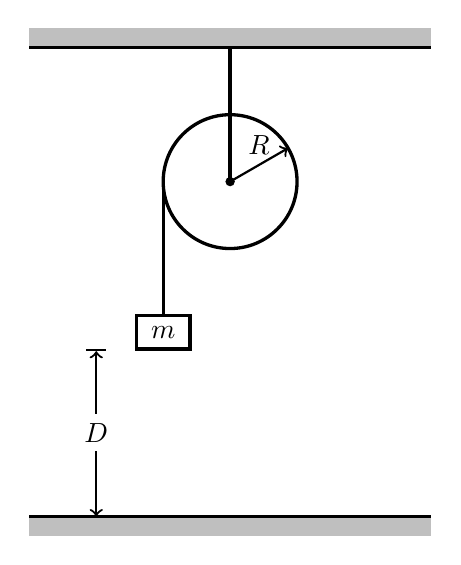
\begin{tikzpicture}[scale=.85]
        \draw[very thick] circle(1);
        \fill circle(.07);
        \draw[very thick](0,0)--(0,2);
        \fill[lightgray](-3,2) rectangle(3,2.3);
        \draw[very thick](-3,2)--(3,2);
        \draw[thick,->,rotate=30](0,0)--(1,0) node[midway,above]{$R$};
        \draw[very thick](-1,0)--(-1,-2);
        \draw[very thick](-1.4,-2) rectangle(-.6,-2.5) node[midway]{$m$};
        \draw[thick,|<->](-2,-2.5)--(-2,-5) node[midway,fill=white]{$D$};
        \fill[lightgray](-3,-5) rectangle(3,-5.3);
        \draw[very thick](-3,-5)--(3,-5);
      \end{tikzpicture}
    \end{center}
  }
  \question A solid disk of unknown mass and known radius $R$ is used as a
  pulley in a lab experiment, as shown above. A small block of mass $m$ is
  attached to a string, the other end of which is attached to the pulley and
  wrapped around it several times. The block of mass $m$ is released from rest
  and takes a time $t$ to fall the distance $D$ to the floor.
  \begin{parts}
    \part Calculate the linear acceleration $a$ of the falling block in terms
    of the given quantities.

    \part The time $t$ is measured for various heights $D$ and the data are
    recorded in the following table.
    \begin{center}
      \begin{tabular}{|c|c|}
        \hline
        $D$ (\si\metre) & $t$ (\si\second)\\\hline
        0.5 & 0.68 \\\hline
        1   & 1.02 \\\hline
        1.5 & 1.19 \\\hline
        2   & 1.38 \\\hline
      \end{tabular}
    \end{center}
    \begin{subparts}
      \subpart What quantities should be graphed in order to best determine the
      acceleration of the block? Explain your reasoning.

      \subpart On the grid below, plot the quantities determined in (b)i,
      label the axes, and draw the best-fit line to the data.
      
      \vspace{.1in}
      \begin{center}
        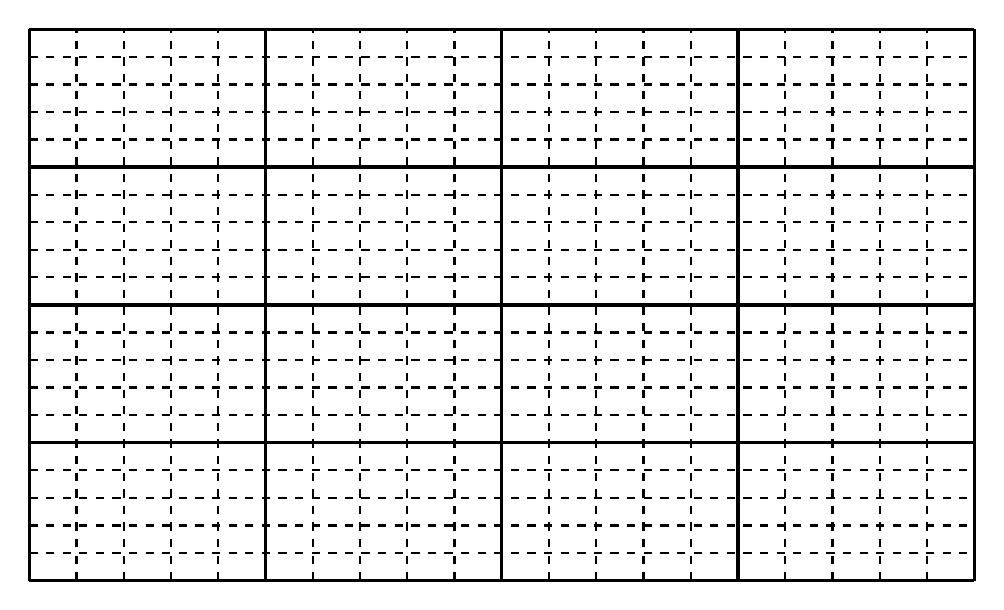
\begin{tikzpicture}[xscale=.6,yscale=.35]
          \draw[thick,dashed] grid(20,20);
          \draw[very thick,step=5] grid(20,20);
        \end{tikzpicture}
      \end{center}\vspace{.2in}
      
      \subpart Use your graph to calculate the magnitude of the acceleration.
    \end{subparts}

    \part Calculate the rotational inertia of the pulley in terms of $m$, $R$,
    $a$, and fundamental constants.

    \part The value of acceleration found in (b)iii, along with numerical
    values for the given quantities and your answer to (c), can be used to
    determine the rotational inertia of the pulley. The pulley is removed from
    its support and its rotational inertia is found to be greater than this
    value. Give one explanation for this discrepancy.
  \end{parts}
  \newpage
  
  \question A uniform ball of radius $r$ rolls without slipping along the
  loop-the-loop track in the figure below. The ball starts at rest at a height
  of $h$ above the bottom of the loop.
  \cpic{.55}{roll-ball}
  \begin{parts}
    \part If it is not to leave the track at the top of the loop, what is the
    least value $h$ can have (in terms of radius $R$ of the loop)?

    \part What would $h$ have to be if, instead of rolling, the ball slides
    without friction?
  \end{parts}
%  \newpage
%  
%  \begin{center}
%    \begin{tikzpicture}[scale=.65]
%      \fill[gray!70] circle(1);
%      \draw[ultra thick,->](-1,4.5)--(-1,0) arc(180:360:1)
%      --(1,2) node[above]{$F_A$};
%      \draw[thick](-1,0) arc(180:0:1);
%      \fill[gray](-5,4.5) rectangle(4,4.9);
%    \end{tikzpicture}
%  \end{center}
%  \question A disk of mass $M =\SI{2.}{\kilo\gram}$ and radius
%  $R=\SI{.10}\metre$ is supported by a rope of negligible mass, as shown
%  above. The rope is attached to the ceiling at one end and passes under the
%  disk. The other end of the rope is pulled upward with a force $F_A$. The
%  rotational inertia of the disk around its center is $MR^2/2$.
%  \begin{parts}
%    \part Calculate the magnitude of the force $F_A$ necessary to hold the disk
%    at rest.
%
%    \uplevel{
%      At time $t=0$, the force $F_A$ is increased to 12 N, causing the disk to
%      accelerate upward. The rope does not slip on the disk as the disk rotates.
%    }
%
%    \part Calculate the linear acceleration of the disk.
%    
%    \part Calculate the angular speed of the disk at $t=\SI{3.}\second$.
%    
%    \part Calculate the increase in total mechanical energy of the disk from
%    $t=0$ to $t=\SI{3.}\second$.
%    
%    \part The disk is replaced by a hoop of the same mass and radius. Indicate
%    whether the linear acceleration of the hoop is greater than, less than, or
%    the same as the linear acceleration of the disk. Justify your answer.
%
%    \vspace{.1in}   
%    \underline{\hspace{.3in}} Greater than\hspace{.2in}
%    \underline{\hspace{.3in}} Less than\hspace{.2in}
%    \underline{\hspace{.3in}} The same as
%  \end{parts}
\end{questions}
\end{document}
